\section{Strømforsyning}
\subsection{Printudlæg}

For at implementere kredsløbet i figur \ref{fig:bil_psu} på side \pageref{fig:bil_psu} er der udarbejdet et PCB layout for strømforsyningen.
Dette kan ses i figur \ref{fig:bil_psu_pcb}. 
Under udlægget af printet er der taget forbehold for at minimere arealet af strømsløjfer, som ligger i forbindelse med den skiftende udgang samt returveje derfra på LM26003. Ydermere er der også forsøgt at give så god elektrisk kontakt som muligt ved hjælp af brede printbaner til de komponenter, som forventes at trække en stor, evt. skiftende, strøm.
Dette kan ses i området omkring 3V udgangen fx, da diode, spole, udgang samt kondensator ligger helt op ad hinanden. 
De kredse, som ligger i forbindelse med tilbagekoblingen til LM26003 ligger på den 'nedre' del af printet for at minimere støjen fra de skarpe flanker på LM26003's udgang (ben 1-3 og 11-13).
Grundet at skolens komponentlager ikke lå inde med keramiske kondensatorer i størrelsen 6.8 $\mu F$ er der i stedet sat 7 parallelkoblede kondensatorer i på hver 1 $\mu F$.

\vfill

\begin{figure}[h]
\centering
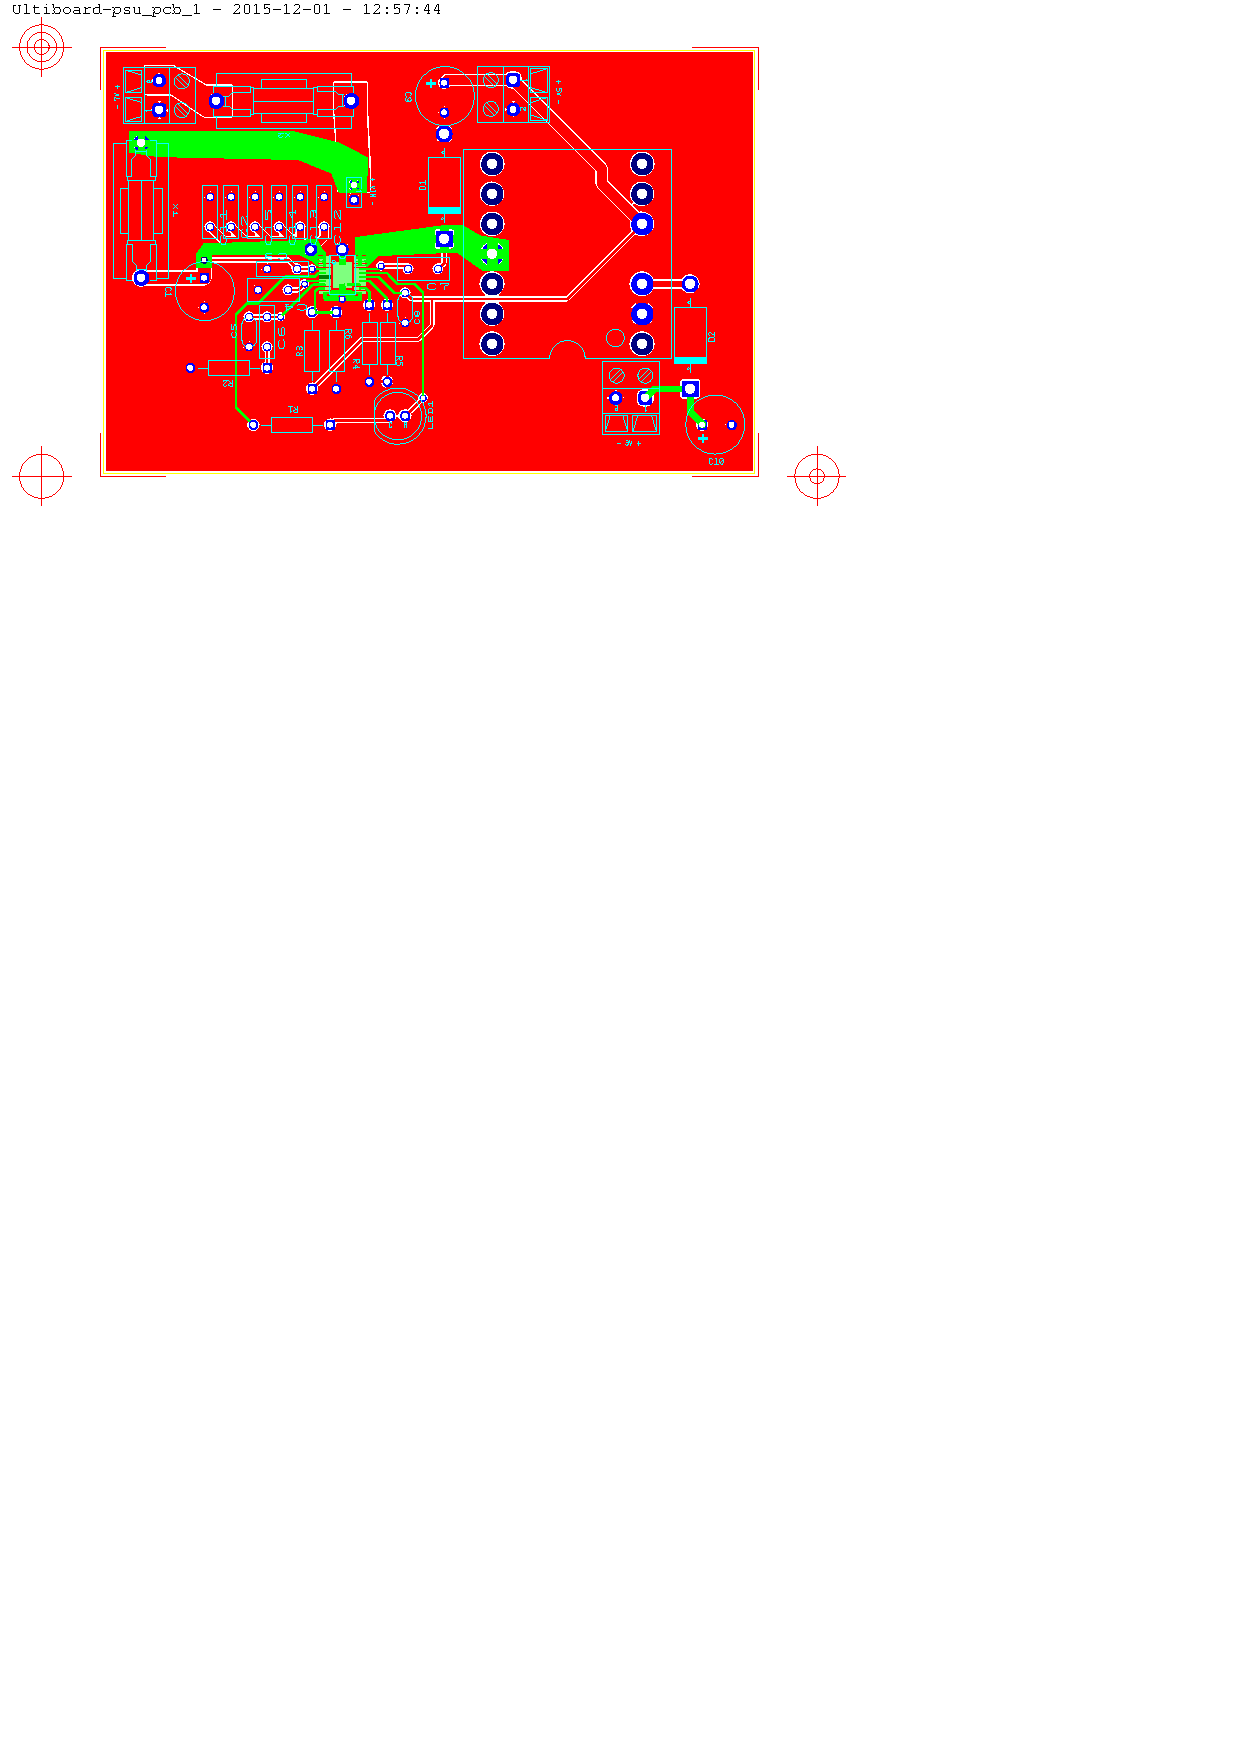
\includegraphics[angle=90,height=\textheight-9cm, clip=true, trim=50 615 234 25]{../fig/diagrammer/bil/psu_pcb_twoside}
\caption{Bilens strømforsyning på PCB}
\label{fig:bil_psu_pcb}
\end{figure}

\clearpage

\subsection{Test}

For at teste strømforsyningen er denne koblet op mod en laboratoriespændingsforsyning indstillet til 7.2V DC.